\documentclass[12pt]{article}
\usepackage{booktabs}
\usepackage{geometry}
\usepackage{enumerate}
\usepackage{setspace}
\usepackage{amsthm}
\usepackage{amsmath,amssymb}
\usepackage{amstext}
\usepackage[hidelinks]{hyperref}
\usepackage{graphicx}
\usepackage{setspace}
\usepackage{wrapfig}
\usepackage{fourier}
\usepackage{indentfirst}

\geometry{a4paper,scale=0.82}
\linespread{1.5}

\newtheorem{definition}{Definition}[section]
\newtheorem{theorem}{Theorem}[section]
\newtheorem{lemma}{Lemma}[section]
\newtheorem{proposition}{Proposition}[section]
\newtheorem{remark}{Remark}[section]
\newtheorem{corollary}{Corollary}[section]

\def\d{\mathrm{d}}
\def\Cov{\mathrm{Cov}}
\def\E{\mathrm{E}}
\def\Var{\mathrm{Var}}
\def\unf#1{\textcolor{blue}{#1}}

\newcommand{\HRule}[1]{\rule{\linewidth}{#1}}

\begin{document}

\title{ \normalsize \textsc{VE401 Term Project}
		\\ [3.0cm]
		\HRule{0.5pt} \\ [0.5pt]
        \vspace*{\baselineskip}
		\LARGE \textbf{\textsc{Verification of Sampling Criterion in Testing for Net Quantity of Prepackages with Fixed Content}}
		\HRule{2pt} \\ [0.5cm]
        \vspace*{\baselineskip}
		\normalsize \today \vspace*{5\baselineskip}}

\date{}

\author{
		Project Group 26 \\ 
        \begin{tabular}{ll}
        \normalsize Meng Yuqi & \normalsize 521370910030  \\
		\normalsize Tanchavalit Ekkanat & \normalsize 521370990007  \\
        \normalsize Liu Yuzhuo & \normalsize 520021910454  \\ 
        \normalsize Zhang Maizhe & \normalsize 521370910157  \\
        \end{tabular}}
        

\maketitle
\thispagestyle{empty}
\newpage
\thispagestyle{empty}

\tableofcontents
\thispagestyle{empty}
\newpage
\pagenumbering{arabic}

\section{Abstract}

\newpage

\section{Introduction}

As prepackaged food production becomes prevalent nowadays, inspection on whether the product contains the same amount of content as labeled becomes an important approach to protect the interests of the consumers. However, there are unavoidable errors in the production, which makes it impossible to ensure that every package produced contains content at least as much as what is specified in the label. It would in turn be unfair to the manufacturers as on average they would have to fill more content when packaging the products. Therefore, a statistically reasonable criterion is called for to resolve this dilemma, so that a general agreement is reached upon on how much error is allowable for a certain batch of production; and a standard is derived from the criterion to specify how the random sampling and inspection should be carried out to determine whether the production satisfies the requirement or not.

In our project, we refer to two specific criterion that is published by Chinese government \cite{JJF2005} and International Organization of Legal Metrology \cite{OIML2016}, respectively, to explain how the "statistically reasonable" is established, and verify whether the sampling plan proposed in the two criteria aligns with the requirements that are specified in their materials. We would first look into the \cite{JJF2005} first and cross-validate using \cite{OIML2016}. A comparison between the two criteria will be made; and an empirical sample carried out by ourselves will be demonstrated for supplement. 

\section{Glossary}

In order to avoid confusion in the subsequent elaboration on the contents, we first specify the meaning of some terminologies; and throughout the report we will align to these expressions.

\begin{itemize}
	\item \textbf{Batch:} the assembly of all products produced whose being accepted or not depends on the samples taken from the batch.
	\item \textbf{Sample:} a fraction of products that are taken from the batch for examination. 
	\item \textbf{Package:} an individual in the sample or in the batch.
\end{itemize}

\section{Criterion of Acceptable Batch and Sample; Scheme of Sampling}

Before we dig into the technical details, we first summarize the requirements that are set in both standards (\cite{JJF2005} and \cite{OIML2016}), on both the whole batch and on samples obtained. Interestingly, although they share the same standard on batches, the criteria that are used for sample testing are quite different.

\subsection{Generally Criterion of Batch and Sample}

First we present two definitions that will be used intensively in subsequent discussions, which are defined in \cite{OIML2016}:

\begin{definition}[$T_1$ Error, $T_2$ error]
    For a given standard $Q$ with the applicable tolerable deficiency $T$, a sample $Q_i$ is said to be of $T_1$ error if
    $$
    Q-2T \leq Q_i < Q-T
    $$
    and is said to be of $T_2$ error if
    $$
    Q_i < Q-2T
    $$
\end{definition}

According to both criteria, the samples from a certain batch should satisfy that
\begin{enumerate}
    \item[(A.1)] The sample mean is no less than the labeled nominal amount.
    \item[(A.2)] The proportion of samples with nominal amount less than the required amount (labeled amount minus the tolerable deficiency) is less than 2.5\%.
    \item[(A.3)] There are no $T_2$ errors in the samples. 
\end{enumerate}
and the inspection process should fulfill the requirement to detect defective batches\footnote{The sequence of presenting the rules is slightly changed so that they are classified in terms of statistic examined, instead of type of errors.}:
\begin{enumerate}
    \item[(B.1)] If a shipment is correctly manufactured, i.e. with $\mu\geq Q$ where $Q$ is the labeled amount, than the probability of this being rejected is less than 0.5\%.
    \item[(B.2)] If the mean of the batch is less than $Q-0.74s$, then 90\% of the time we can spot it out (and reject that).
    \item[(B.3)] If the proportion of $T_1$ error is no more than 2.5\%, then the probability of it being rejected is no more than 5\%.
    \item[(B.4)] If the proportion of $T_1$ and $T_2$ error combined is 9\%, then 90\% of the time we can spot it out (and reject that).
\end{enumerate}
with (B.1,2) specifying the requirement of the mean and (B.3,4) specifying the requirement of the variance (as the restriction of Type I and II Errors are a restraining factor of the variance of the production). All these rules will be elaborated on in the next section.

\subsection{Scheme of Sampling}

Although the organizing ideas in both criterion are the same, the suggestions they provided in obtaining the samples are quite different. The major difference is in how the sample size $n$ should relate to the size of the population (size of batch) $N$. 

\subsubsection{Scheme of Sampling in \cite{JJF2005}}

In \cite{JJF2005}, the choice of sample size $n$ should be selected according to the following table\footnote{Entry ``Log$(N)$'' and ``Log$^2(N)$'' takes the lower bound of $N$ in each row}:

\begin{table}[htbp]
    \centering
    \begin{tabular}{ccccc}
        \toprule
        $N$ (Batch Size) & $n$ (Sample Size) & Log$(N)$ & Log$^2(N)$ & $n/\text{Log}^2(N)$ \\
        \midrule
        1-10 & $N$ & N/A & N/A & N/A \\
        11-50 & 10 & 2.40 & 5.75 & 1.74 \\
        51-99 & 13 & 3.93 & 15.46 & 0.84 \\
        100-500 & 50 & 4.61 & 21.21 & 2.36 \\ 
        501-3200 & 80 & 6.22 & 38.65 & 2.07 \\
        $>$3200 & 125 & 8.07 & 65.14 & 1.92 \\
        \bottomrule
    \end{tabular}
    \caption{Designated Sample Size $n$ Given Batch Size $N$}
\end{table}

There is a general trend in the selection of $n$: the larger $N$ is, the smaller the incremental step of $n$ takes. This much resembles the behavior of a logarithm-like function; therefore of our interest we list statistics of Log$(N)$ as well. And it actually should: heuristically, the sample size $n$ should be be able to organize changes in batch size $N$ faster than linearly, and logarithm seem to be a good fit in this case. 

Although we have to admit that logarithm is a quite brutal, unverified and not so approximate modelling of the data, it could yield some insights. Specifically, we can see all rows applicable to doing the division $n/\text{Log}^2(N)$ except for the third one yields a results of 2.0 $\pm$ 0.4. In later parts we will verify whether the criterion listed here makes full sense. 

\subsubsection{Scheme of Sampling in \cite{OIML2016}}

We similarly present the table specified in \cite{OIML2016}\footnote{In \cite{OIML2016} there are more detailed table listed in Appendix I; but in order to make the discussion more concise and follow the realistic criterion more closely, we use the table listed in page 18.} according to which the sample size should be chosen:

\begin{table}[htbp]
    \centering
    \begin{tabular}{ccccc}
        \toprule
        $N$ (Batch Size) & $n$ (Sample Size) & Log$(N)$ & Log$^2(N)$ & $n/\text{Log}^2(N)$ \\
        \midrule
        1-20 & $N$ & N/A & N/A & N/A \\
        21-40   & 32 & 3.04 & 9.27  & 3.45 \\
        41-60   & 35 & 3.71 & 13.79 & 2.54 \\
        61-80   & 47 & 4.11 & 16.90 & 2.78 \\
        81-100  & 49 & 4.39 & 19.31 & 2.54 \\
        100-200 & 64 & 4.61 & 21.21 & 3.01 \\
        200-300 & 67 & 5.30 & 28.07 & 2.39 \\
        300-400 & 81 & 5.70 & 32.53 & 2.49 \\
        400-500 & 81 & 5.99 & 35.90 & 2.27 \\
        $>$500  & 98 & 6.21 & 38.62 & 2.54 \\
        \bottomrule
    \end{tabular}
    \caption{Designated Sample Size $n$ Given Batch Size $N$}
\end{table}

The statistic generally falls into a centered region of 2.9 $\pm$ 0.6. There seem to be some anomaly in the case where $N$ is in the range 401-500; but the difference is small and insufficient for drawing any conclusion. Further results can not be drawn from this approximation as it is quite intuitive and not yet verified. We can vaguely sense that this table is less likely to be wrong than \cite{JJF2005}; but further investigations are required, which we will present in juxtaposition with the that of the previous table. 

\section{Hypothesis Testing}

The statistic foundation of formulating the probability of various situations is hypothesis testing. In order to rigorously conduct discussions on the probability of accepting or rejecting a certain package, we need to formalize them using Neyman-Pearson Decision Theory \cite{Ho2023}, accept or reject according to the sample falling into critical region or not, and comment on Type II Error and the power of the test. We will resolve these problems in this section.

Besides explaining the source of the statistics listed in the table, we would also like to look into the symmetry in Neyman-Pearson Decision Theorem. The criterion gives a test using central $T$-distribution where $\mu=\mu_0$ where $Q$ is the sample mean and $Q_0$ is the labeled amount is the boundary case. What conclusion will be drawn if the test statistic is not the same for cases $H_0$ and $H_1$? The above question will be discussed in depth in the following subsections.

\subsection{Overview of Approach Using Neyman-Pearson Decision Theorem}

In Neyman-Pearson Decision Theorem, the null hypothesis and the alternative hypothesis should be symmetric in terms of being accepted and rejected. However, there are some asymmetries in the designation of the hypotheses as the requirements of probability of conducting a Type I Error and that of conducting a Type II Error are not necessarily the same. 

We first state explicitly the Neyman-Pearson Test that we are conducting. According to the criterion (A.1) and (B.3), the boundary cases are either the batch is of mean $Q$ exactly equal to the labeled amount $Q_0$, or it has a shortfall of at least $\sigma$ (that is, of at least $T_1$ Error). We set up the null hypothesis and alternative hypothesis to be
\begin{equation}\label{hypothesis1}    
    H_0 : Q\geq Q_0 \quad\quad\quad\quad H_1 : Q\leq Q_0 - \sigma
\end{equation}
and if we manage to reject $H_0$ at certain (low) level of significance, we would conclude that the batch does not satisfy the requirement. 

In order to take into account potential differences in both approaches, in the following discussion we will first do an ordinary Neyman-Pearson Test and then have a discussion on whether we could switch $H_0$ and $H_1$; and why we are not using that in this case

\subsection{Testing for $H_0$ Using Student's $T$-Distribution}

First we perform the test on the boundary case for $H_0$, i.e. following the ordinary method for performing a Neyman-Pearson Test. 

As we are performing test in the case where the variance us unknown, the test statistic with mean of the process $\mu$ is 
$$
T_{n-1} = \dfrac{\overline{X} - \mu}{S/\sqrt{n}}
$$
should follow a $T$-distribution with $n-1$ degrees of freedom. Therefore, a 100($1-\alpha$)\% confidence interval for the statistic is
$$
\left[\overline{Q}-\dfrac{t_{\alpha,n-1}S}{\sqrt{n}},\infty\right)
$$
Suppose that the random variable (process) generating all the samples yields a mean of exactly $Q_n$, since $\alpha = 0.005$ and $n$ according to the table in \cite{JJF2005} is desired, we would like 99.5\% of the times when a sample is generated using the process, it will fall above the threshold. Then, the lower bound of $\overline{q}$ is the lower bound of a 99.5\% confidence interval for the test statistic $T_{n-1}$ when $\mu = Q_n$, which gives
$$
\dfrac{\overline{Q} - Q_0}{S/\sqrt{n}} \geq -t_{0.995, n-1} \quad\Leftrightarrow\quad \overline{Q}\geq Q_0-\dfrac{S}{\sqrt{n}}t_{0.995, n-1}
$$ 
which corresponds to $\lambda\cdot s$ in the third column of the table. Note that the $t_{0.995}$ in the table actually refers to $t_{0.995, n-1}$, where the degrees of freedom is omitted in the table. Using mathematica we easily verify that our calculation aligns with the form by comparing the value of $\frac{t_{0.995, n-1}}{\sqrt{n}}$ and $\lambda$:

\begin{table}[htbp]
    \centering
    \begin{tabular}{ccc}
        \toprule
        $n$ & $\frac{t_{0.995, n-1}}{\sqrt{n}}$ & $\lambda$ \\
        \midrule
        10 & 1.028 & 1.028 \\
        13 & 0.848 & 0.848 \\
        50 & 0.379 & 0.379 \\
        80 & 0.295 & 0.295 \\
        125 & 0.234 & 0.234 \\
        \bottomrule
    \end{tabular}
    \caption{Verification of Equality between $\lambda$ and $\frac{t_{0.995, n-1}}{\sqrt{n}}$}
\end{table}

Up to this point, we have determined the critical region for various cases given $\alpha$ value. We will now seek to obtain the probability of conducting a Type II Error, i.e. $\beta$.

\subsection{Power Analysis Using Noncentral $T$-Distribution}

If the mean of the sample is not the same as the value declared in the null hypothesis $Q_0$, the statistic ceases to follow a $T$-distribution. In order to analyze the statistic in this case, we introduce the \textbf{Noncentral $T$-Distribution} for further discussions. 

\begin{definition}[Noncentral $T$-Distribution]
    Suppose that $Z$ is a standard normal variable and $\chi_{\gamma}^2$ follows a chi-squared distribution with $\gamma$ degrees of freedom, with $\delta$ a constant real number. Then
    $$
    T_{\gamma, \delta} := \dfrac{Z + \delta}{\sqrt{\chi_{\gamma}^2/\gamma}}
    $$
    is defined to follow a noncentral $T$-distribution with $\gamma$ degrees of freedom and non-centrality $\delta$. 
\end{definition}

In order to grasp how the non-centrality influences the behavior of probability density function (PDF), we plot the PDF of noncentral $T$-distribution with different centrality together with those of different degrees of freedom. The result is shown as below, with $\gamma$ denoting the degrees of freedom and $\delta$ denoting the non-centrality\footnote{Generated using Mathematica, with source code listed in \ref{mmacode}}:

\begin{figure}[htbp]
    \centering
    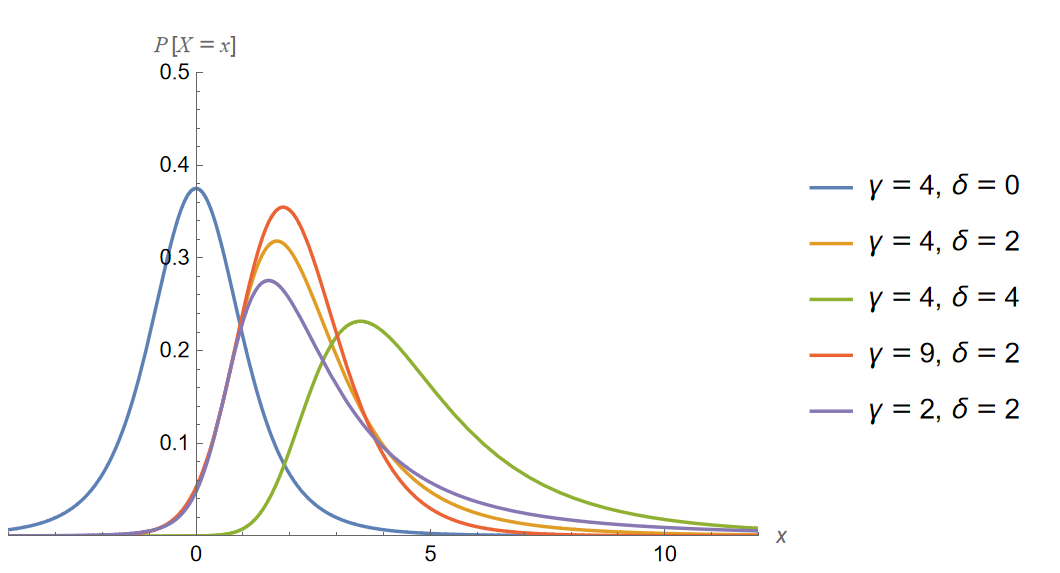
\includegraphics[scale=0.65]{img/pdf_noncentral_t.png}
    \caption{Probability Density Function of Noncentral $T$-Distribution with Various Parameters}
\end{figure}

From the figure we can infer some properties of noncentral $T$-distribution: similar to $T$-distribution, it is uni-modal, but has a skewed behavior towards the direction of non-centrality; and the skewing effect increases as the non-centrality increases. Again similar to $T$-distribution, as the degrees of freedom increases noncentral $T$-distribution behaves more and more like normal distribution with mean the same as the non-centrality. This makes sense as with the sample size increasing, the unbiased estimator for sample variance will have a closer and closer approximation of the actual variance $\sigma^2$, in which case we have exactly the normal distribution.

Using this, we now seek to use this for power analysis. Manipulating the expressions, we have
\begin{equation}\label{noncentralt}
    T_{n-1,\mu\sqrt{n}/\sigma}=\frac{\frac{\Bar{X}-\mu}{\sigma/\sqrt{n}}+\frac{\mu}{\sigma/\sqrt{n}}}{\sqrt{\frac{(n-1)S^2}{\sigma^2}\frac{1}{n-1}}}=\frac{\Bar{X}}{S/\sqrt{n}}
\end{equation}
which follows a non-central student T-distributed with $n-1$ degrees of freedom and $\frac{\mu\sqrt{n}}{\sigma}$ non-centrality. That is, if the sample is taken from a batch that does not has mean $\mu$, its distribution will be like this. In this case, we can also interpret $\mu$ as the difference between the actual mean and the mean that we estimate (or the mean that is stated in the null hypothesis).

Since we have obtained the critical region to be
$$
(-\infty, t_{0.995,n-1})
$$
we will calculate $\beta$ as the integral of the noncentral $T$-distribution on the complementary of the critical region, which can be evaluated via
$$
\beta = \int_{-t_{0.005, n-1}}^{\infty} f_{T_{n-1, \frac{\mu\sqrt{n}}{\sigma}}}(x) \d x
$$
As the $\beta$ value is only related to $n$ and the quotient of $\mu$ and $\sigma$, we could express the difference in mean using the multiples of sigma, which gives the Operating Characteristic (OC) Curve as below\footnote{Generated using Mathematica, with source code listed in \ref{mmacode}}:

\begin{figure}[htbp]
    \centering
    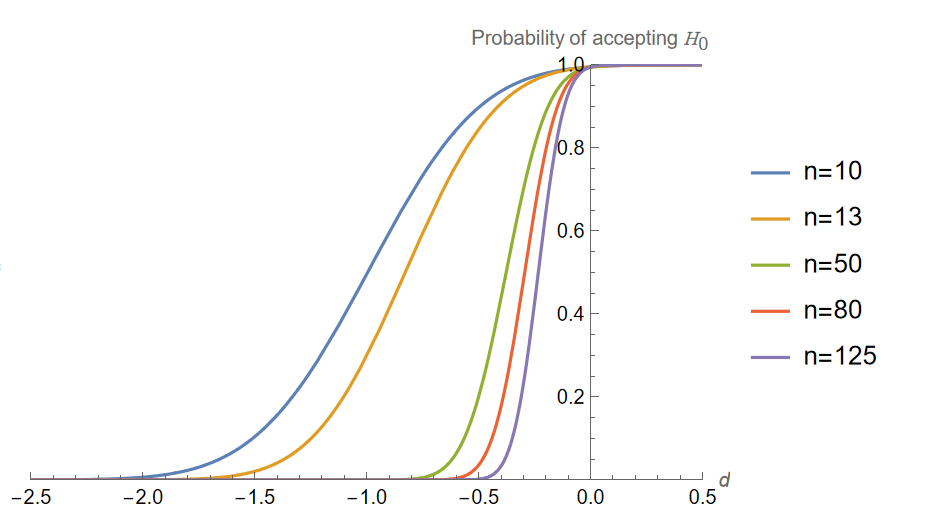
\includegraphics[scale=0.6]{img/oc_noncentral_t.png}
    \caption{OC Curve for One-Tailed Test of Noncentral $T$-Distribution with n Specified in Table 4.3.2}
\end{figure}

\noindent where we have adopted the abscissa to be
$$
d := \dfrac{\mu - \mu_0}{\sigma}
$$
and the ordinate to be the probability of accepting $H_0$ since by definition
$$
P[\text{Accept } H_0] = 1 - P[\text{Reject }H_0]
$$
Without calculating explicitly, we can claim that the test is fairly powerful. Suppose that the non-centrality is of $\sigma$, i.e. the mean of the batch is of shortfall of one standard deviation, for sample size $n\geq 50$ the probability of detecting this is almost 1. Even for the requirement (B.2) that we should spot batches with mean less than or equal to $Q_0 - 0.74\sigma$ ($\delta = Q_0 - 0.74\sigma$), for $n\geq 50$ we can satisfy the requirement as the OC Curve approaches zero. The explicit evaluation of $\beta$ justifies the intuition:

\begin{table}[htbp]
    \centering
    \begin{tabular}{ccc}
        \toprule
        $n$ & $1-\beta\mid\delta = Q_0 - \sigma$ & $1-\beta\mid\delta = Q_0 - 0.74\sigma$ \\
        \midrule
        10 & 0.504 & 0.256 \\
        13 & 0.701 & 0.393 \\
        50 & 1.000 & 0.993 \\
        80 & 1.000 & 1.000 \\
        125 & 1.000 & 1.000 \\
        \bottomrule
    \end{tabular}
    \caption{Power of Testing Using Noncentral $T$-Distribution of Different Non-centrality with Varying $n$}
\end{table}

\noindent Note that we table $1-\beta$ instead of $\beta$ to align with the OC Curve and to show the power of the test. The evaluations give us concrete evidence that the test is powerful enough for $n\geq 50$.

\subsection{Why don't We Switch $H_0$ and $H_1$?}

In the lectures \cite{Ho2023} we have concluded that Neyman-Pearson Decision Theory yields symmetric results with respect to $H_0$ and $H_1$, i.e. it does not matter whether we choose $H_0$ to be $Q \geq Q_0$ or $Q \leq Q_0 - \sigma$. Therefore, we will try the other way round; we set up the hypotheses according to (B.2):
\begin{equation}\label{hypothesis2}
    H_0 : Q\leq Q_0 - 0.74\sigma \quad\quad\quad\quad H_1 : Q\geq Q_0
\end{equation}
and conduct Neyman-Pearson Hypothesis Testing as usual. Theoretically the results should be the same. We will then comment on why we choose \eqref{hypothesis1} for the test. 

Suppose that the test statistic is on the boundary value of $H_0$. Then the statistic should satisfy the following conditions according to \eqref{noncentralt}:
$$
T_{n-1,-0.74\sqrt{n}}=\frac{\frac{\Bar{X}-\mu}{\sigma/\sqrt{n}}+\frac{\mu}{\sigma/\sqrt{n}}}{\sqrt{\frac{(n-1)S^2}{\sigma^2}\frac{1}{n-1}}}=\frac{\Bar{X}}{S/\sqrt{n}}\quad\sim\quad \tilde{T}(n-1,-0.74\sqrt{n})
$$
where $\tilde{T}(\gamma, \delta)$ denotes a noncentral $T$-distribution with degrees of freedom $\gamma$ and non-centrality $T$. Since we would like to not reject $H_0$ in 90\% of the cases, we have the critical region
$$
\left[t_{0.9,n-1,-0.74\sqrt{n}}\right)
$$
and the probability to conduct a Type II Error
$$
\beta := \int_{-\infty}^{t_{0.9,n-1,-0.74\sqrt{n}}}f_{T_{n-1}}(x) \d x
$$ 
And we have $\beta$ for this specific case with different $n$s:

\begin{table}[htbp]
    \centering
    \begin{tabular}{ccc}
        \toprule
        $n$ & $1-\beta\mid\delta = Q_0 - 0.74\sigma$ \\
        \midrule
        10 & 0.839 \\
        13 & 0.902 \\
        50 & 1.000 \\
        80 & 1.000 \\
        125 & 1.000 \\
        \bottomrule
    \end{tabular}
    \caption{Power of Using the Noncentral Case as Null Hypothesis with Varying $n$}
\end{table}

\noindent which indicates that the test is quite powerful for $n\geq 50$, similar to the previous test that we have presented. Therefore, up to this point we can conclude with fairly good confidence that when performing Neyman-Pearson Test in this case, treating one hypothesis as either the null hypothesis or as the alternative hypothesis are equivalent.

However, there are reasons for adopting the null hypothesis as the centered one instead of doing this in the alternative way described in this section. We also did not provide the OC Curves, which results from reasons described below. The two main reasons are the difference in obtaining the referential numbers, and the asymmetry between obtaining $\alpha$ and $\beta$ in the process. 

\begin{itemize}
    \item Noncentral $T$-distribution is much harder to calculate and behaves much less nicely. If one wants to provide a table for tests using noncentral $T$-distribution with $P$-values, one would need to perform the calculations on both sides as noncentral $T$-distribution is not symmetric. Moreover, the OC Curves for noncentral $T$-distribution is much harder to calculate as the PDF of that is more complex. That is the reason why we did not provide the OC Curves: Mathematica performed the calculation for more than half an hour without spitting any curve.
    \item In this case we have much stronger restriction on the error that can be conducted in judging $alpha := \overline{Q} \geq Q_0$ than on judging $\beta := \overline{Q} \leq Q_0 - 0.74\sigma$. Therefore, if we determine $\beta$ in the first place, the expression for $\alpha$ will be an integral which is much harder to evaluate. Moreover, even if one has an OC Curve for this test, it would be nearly useless as it is hard to tell which value corresponds to $\alpha = 0.995$ unless the graph is zoomed in extraneously and in extreme precision. 
\end{itemize}

Therefore, it would be better to conduct Neyman-Pearson Test with the boundary case following $T$-distribution rather than doing that based on cases following noncentral $T$-distribution, as is described in the criterion \cite{JJF2005} and \cite{OIML2016}.

\section{Verification of Sample Size $n$ and Type I Error Tolerance}

In this section, we would finally address the problem that was raised when we first look into the criterion: do the sampling size $n$ specified in each criterion conforms to the general requirements that are described in corresponding standard. We would conduct the verification in three approaches: a simple alignment test; a verification based on calculation introduced in \cite{OIML2016}; and a final one referring to the organizing requirements (B.1) through (B.4) where we refer the calculations to the Appendix F in \cite{OIML2016}. In the last section we would also verify whether the standard of tolerable Type I defectives described in both \cite{JJF2005} and \cite{OIML2016} can satisfy the requirements.

\subsection{Alignment Test of $n$ with Inference on Proportions}

In discussions in this section, we will introduce a method to verify mere alignment of standard in different region that $N$ falls into; and we will compress the information of the samples to be qualified or not. After introducing the method, we will verify whether there is alignment in tables of both criterion.

As the information is compressed quite a lot, this is only a preliminary test and we will present more precise tests in later sections. However, there are quite a bit insights that this method can yield, which will be elaborated as follows.

\subsubsection{Introduction to Methods of Comparing Proportion}

First of all, if the total size of shipment is quite small (less than or equal to 10), sampling is not necessary since examining all the individual package is sufficient enough and not costly. 

For other cases, we are trying to make an inference on the proportion of the samples that do not fall short in the amount of product. But instead of having samples generating from a repeatable process, we are taking a portion from the population without replacing it. This causes a perturbation on the resulting sample variance. Therefore, in order to determine the appropriate sample size, we need to first investigate the sample variance in this case. We quote the following theorem:

\begin{theorem}[Sample Variance for Sampling without Replacement]
    Suppose that we draw $n$ samples from a population of size $N$ and variance $\sigma$. Then the sample variance is
    $$
    \Var(\overline{X}) = \dfrac{\sigma^2}{n}\cdot\dfrac{N-n}{N-1}
    $$
\end{theorem}

We refers to \cite{Sampling} for the proof

\begin{proof}
    Recall how the proof is conducted in the case where $N$ is infinite:
    $$
    \Var[\overline{X}] = \Var\left[\frac{1}{n}\sum\limits_{k=1}^n X_k\right] = \dfrac{1}{n^2} \sum_{1\leq i,j\leq n}\Cov[X_i, X_j]
    $$
    In the case where $N$ is infinite, the influence of replacement is almost zero; and we could conclude that all the $X_i$s are independent, which gives 
    $$
    \Cov[X_i, X_j] = \begin{cases}
        \Var[X_i] &, i = j\\
        0 &, i\neq j 
    \end{cases}
    $$
    But if $N$ is finite, the covariances should be calculated manually. Denote $\xi_i$ to be the values of the samples, $n_i$s the number of samples sharing value $\xi_i$ and $p_i$ the probability of obtaining value $\xi_i$, we have
    \begin{align*}
        \E[X_1 X_2] & = \sum\limits_{i, j}\xi_i \xi_j p_{ij} \\
                    & = \sum\limits_{i}\xi_i p_i \sum\limits_{j} \xi_j \frac{p_{ij}}{p_i} \\
                    & = \sum\limits_{i}\xi_i p_i \left(\sum\limits_{j}\left(\xi_j\frac{N p_j}{N-1}\right) - \frac{\xi_i}{N-1} \right) \\ 
                    & = -\frac{1}{N-1}\underset{\E[X^2]}{\underbrace{\sum\limits_{i}\xi_i^2 p_i}} + \frac{N}{N-1}\left(\sum\limits_{j}\xi_j p_j\right)^2 \\
                    & = -\frac{1}{N-1}\left(\sigma^2 + \mu^2\right) + \frac{N}{N-1}\mu^2 \\
                    & = -\frac{1}{N-1}\sigma^2 + \mu^2
    \end{align*}
    which gives the covariance of two random samples
    $$
    \Cov[X_i, X_j] = \E[X_i X_j] - \E[X_i]\E[X_j] = -\frac{1}{N-1}\sigma^2
    $$
    and the variance of $\overline{X}$:
    $$
    \Var[\overline{X}] = \frac{1}{n}\sigma^2 + \frac{n-1}{n}\Cov[X_i, X_j] = \dfrac{\sigma^2}{n}\cdot\dfrac{N-n}{N-1}
    $$
\end{proof}

Then we can infer the adequate size of sample for inference on proportion given that the population is finite with size $N$. 

\begin{theorem}[Sample Size for Finite Population]
    For a sample retrieved from a population of size $N$, to ensure the margin of error (half of the width of confidence interval) $d$ at confidence level $\alpha/2$ for two-sided test, we need the sample size $n$ to be at most
    \begin{equation}\label{ssfinite}
    n\approx \dfrac{z_{\alpha/2}N}{4d^2(N-1)+z_{\alpha/2}}
    \end{equation}
\end{theorem}

\begin{proof}
    The confidence interval of this estimation for the proportion is given as
    $$
    p = \hat{p}\pm z_{\alpha/2} \sqrt{\hat{p}(1-\hat{p})\cdot \dfrac{N-n}{n(N-1)}} =: \hat{p} \pm d
    $$
    Requiring $d\geq z_{\alpha/2} \sqrt{\hat{p}(1-\hat{p})\cdot \frac{N-n}{n(N-1)}}$ gives
    $$
    n\geq \dfrac{z_{\alpha/2}\hat{p}(1-\hat{p})N}{d^2(N-1)+z_{\alpha/2}\hat{p}(1-\hat{p})} = \dfrac{z_{\alpha/2}N}{\frac{d^2(N-1)}{\hat{p}(1-\hat{p})}+z_{\alpha/2}}
    $$
    where since $\hat{p}(1-\hat{p})\leq\frac{1}{4}$ the right hand side is bounded above by
    $$
    \dfrac{z_{\alpha/2}N}{\frac{d^2(N-1)}{\hat{p}(1-\hat{p})}+z_{\alpha/2}} \leq \dfrac{z_{\alpha/2}N}{4d^2(N-1)+z_{\alpha/2}}
    $$
    which gives the minimal size of samples to ensure margin of error $d$
    $$
    n\geq \dfrac{z_{\alpha/2}N}{4d^2(N-1)+z_{\alpha/2}}
    $$
\end{proof}

With these tools at hand, we will now look into both criteria and verify whether the margin of error $d$ is consistent among all the cases.

\subsubsection{Verification of \cite{JJF2005}}

The choice of sample size $n$ based on knowledge of population size $N$ of \cite{JJF2005} is demonstrated in the following table. If the choices of numbers are reasonable, using \eqref{ssfinite} with $z_{\alpha/2} = z_{0.995} = 2.575$ we should see that the estimated $d$ values are consistent. 

\begin{table}[htbp]
    \centering
    \begin{tabular}{ccc}
        \toprule
        $N$ & $n$ & Estimated $d$-value \\
        \midrule
        1-10 & $N$ & N/A \\
        11-50 & 10 & [0.08, 0.23] \\
        51-99 & 13 & [0.19, 0.21] \\
        100-500 & 50 & [0.08, 0.11]\\ 
        501-3200 & 80 & [0.08, 0.09]\\
        $>$3200 & 125 & [0.08, 0.09] \\
        \bottomrule
    \end{tabular}
    \caption{Tabulated Values for Population Size $N$ and Corresponding Sample Size $n$ in \cite{JJF2005}}
\end{table}

with which we have the conclusions

\begin{itemize}
    \item The test is organized aiming at tolerance of defective rate for large shipments ($N > 100$) of at most 
    $$
    D = d_{\text{test}} + d_{\text{tolerance}} = 11\% + \frac{5}{80} = 17\%
    $$
    where $d_{\text{test}}$ is the margin of error for the test, which is at most 0.11 for $N > 100$, and $d_{\text{tolerance}}$ is the tolerable defective rate in the samples examined, which is at most $5/80$ for $N\in[501, 3200]$. 
    \item For small shipments $N \leq 100$, the defective rate allowed can be as high as
    $$
    D = d_{\text{test}} + d_{\text{tolerance}} = 21\% + \frac{1}{13} = 29\%
    $$
    with the same notation. Specifically, for $N\in[51, 99]$ the lower bound of largest allowed defective rate is 0.19, which is a relatively high defective rate. This choice of design may result from avoiding separating into too many cases for small $N$ or reasons specific with products with small shipments, or may be just an error in setting up the criterion.
    \item In order to ensure the coherence exhibited in the rules, we suggest that the \textbf{$n$ for $N$ in 51-99 should be changed into 32}, which is solved with $d=0.08$ using \ref{ssfinite}. In following discussions on this table we will comment on the result with calibrated $n$ value separately besides using the originally tabled value. 
\end{itemize}

\subsubsection{Verification of \cite{OIML2016}}

Similarly, we refer to Table 2 in \cite{OIML2016} to calculate the allowed margin of error $d$ in different $N$s using \eqref{ssfinite} with $z_{\alpha/2} = z_{0.995} = 2.575$. The results are as shown in the table below:

\begin{table}[htbp]
    \centering
    \begin{tabular}{ccc}
        \toprule
        $N$ & $n$ & Estimated $d$-value \\
        \midrule
        1-20 & $N$ & N/A \\
        21-40 & 32 & [0.00, 0.06] \\
        41-60 & 35 & [0.05, 0.09] \\
        61-80 & 47 & [0.06, 0.08]\\ 
        81-100 & 49 & [0.07, 0.08]\\ 
        101-200 & 64 & [0.06, 0.08]\\ 
        201-300 & 67 & [0.08, 0.09]\\ 
        301-400 & 81 & [0.07, 0.08]\\ 
        401-500 & 81 & [0.08, 0.08]\\ 
        $>$501 & 98 & [0.07, 0.08] \\
        \bottomrule
    \end{tabular}
    \caption{Tabulated Values for Population Size $N$ and Corresponding Sample Size $n$ in \cite{OIML2016}}
\end{table}

In the test we can see that the margin of error $d$ is generally organized arount 0.08, which is quite consistent. Therefore, we could claim that there should not exist major errors in choosing the $n$ value according to the batch size $N$ given in \cite{OIML2016}. 

\subsection{Test of $n$ Using Sample Mean}

The criterion published 2016 \cite{OIML2016} specifies how the choice of $n$ should be determined given the batch size $N$. We quote the derivation of the choice here. Since \cite{OIML2016} intrinsically follows this criterion, after presenting the derivation we will simply verify whether the criterion given in \cite{JJF2005} pass this test. 

\begin{theorem}
    In order to satisfy the requirement specified by (B.2), the statistic should satisfy that
    \begin{equation}\label{samplemean}
        \sqrt{\dfrac{n(N-1)}{N-n}} \geq \dfrac{t_{0.1,n-1} - t_{0.995,n-1}}{0.74}
    \end{equation}
\end{theorem}

\begin{proof}
    Using the approximation that $s\approx\sigma$, suppose that for the lot being tested is of mean $Q = Q_0 - 0.74\sigma$, then the sample mean should follow the following distribution:
    $$
    \overline{Q} \sim N\left( -0.74\sigma, \dfrac{\sigma^2}{n}\left( \dfrac{N-n}{N-1} \right) \right)
    $$
    By criterion (B.3), we require
    $$
    P\left[ \overline{Q} < st_{0.995, n-1}\sqrt{\dfrac{N-n}{n(N-1)}} \right] \geq 0.9
    $$
    where the left hand side can be simplified by again using the approximation $s\approx\sigma$
    $$
    P\left[ \overline{Q} < st_{0.995, n-1}\sqrt{\dfrac{N-n}{n(N-1)}} \right] \approx P\left[ T_{n-1} < t_{0.995,n-1} + 0.74\sqrt{\dfrac{n(N-1)}{N-n}} \right]
    $$
    Apply proper substitution and we have
    $$
    \sqrt{\dfrac{n(N-1)}{N-n}} \geq \dfrac{t_{0.1,n-1} - t_{0.995,n-1}}{0.74}
    $$
\end{proof}

Since the requirement ($B.3$) is shared by \cite{JJF2005} and \cite{OIML2016}, we would expect that criterion in \cite{JJF2005} would also satisfy \eqref{samplemean}. Thereby we table out all the statistics and do a comparison:

\begin{table}[htbp]
    \centering
    \begin{tabular}{cccc}
        \toprule
        $N$ & $n$ & $\frac{n(N-1)}{N-n}$ & $\frac{t_{0.1,n-1} - t_{0.995,n-1}}{0.74}$ \\
        \midrule
        1-10 & $N$ & N/A & N/A \\
        11-50 & 10 & [12.25, 100] & 6.26 \\
        51-99 & 13 & [14.8, 17] & 5.96 \\
        100-500 & 50 & [55, 99] & 5.37 \\ 
        501-3200 & 80 & [82, 95] & 5.31 \\
        $>$3200 & 125 & [125, 130] & 5.28 \\
        \bottomrule
    \end{tabular}
    \caption{Tabulated Values for Population Size $N$ and Corresponding Sample Size $n$ Together with Statistics mentioned in \eqref{samplemean}}
\end{table}

In the table we can see that $\frac{n(N-1)}{N-n}$ is significantly larger than $\frac{t_{0.1,n-1} - t_{0.995,n-1}}{0.74}$, which indicates that \cite{JJF2005} does not have significant defect in detecting errors in the mean of the sample.

\subsection{Verification of Type I Error Tolerance; Cross Reference of Sample Size $n$}

We finally look into the where does the number of tolerable defects in the table comes from. Since the measurement of errors is more of a restriction on the variance given that other criteria (A.1) have applied strict restrictions on the mean. Therefore, in this section we will mainly focus on (B.3) and (B.4); and conduct calculations correspondingly.

As the general criterion does not specify the number of $T_1$ errors allowed in the inspection, the number depends on the actual size of shipment and needs to be determined accordingly. We now seek to verify the correctness of the tolerable $T_1$ errors in the form. 

In the following discussion, we denote $N_1, N_2$ to be the number of sampled packages of $T_1$ error and $T_2$ error in the population, with $n_1, n_2$ the corresponding number of sampled packages in the samples. The goal is to find the maximum tolerable numbers of $T_1$ error in the samples $k_{N}$ given the size of the whole batch $N$. Some of the discussion results are quoted from Appendix F in \cite{OIML2016}.

\subsubsection{Requirement of (B.3)}

If a sample is not rejected according to the criterion, it must satisfy that $P[Q_i < Q - T] \leq 0.025$, i.e. 
$$
\dfrac{Q_i - Q}{T/z_{0.025}} = \dfrac{Q_i - Q}{T/1.96}\sim N(0,1)
$$
Therefore, we require that
\begin{equation}\label{b3}
    P[n_1\leq k, n_2 = 0\mid N_1 = 0.025N, N_2 = 0] \geq 0.95
\end{equation}

\subsubsection{Requirement of (B.4)}

Suppose that 9\% of the batch evaluates to be less than $T$, the distribution of $Q$ evaluates to be
$$
\dfrac{Q_i - Q}{T/z_{0.09}} = \dfrac{Q_i - Q}{T/1.34}\sim N(0,1)
$$
Then 
$$
N_2 = P[\dfrac{Q_i - Q}{T/1.34} < -2.68] = P[Z < -2.68] = 0.0037N, \quad N_1 = [-2.68\leq Z < 1.34] = 0.0863N
$$
The requirement becomes
\begin{equation}\label{b4}
    P[n_1\leq k, n_2 = 0\mid N_1 = 0.0863N, N_2 = 0.0037N] < 0.1
\end{equation}

\subsubsection{Verification of Tolerable $T_1$ Errors}

Since $n_1$ and $n_2$ are chosen simultaneously, they follow a bi-variate hyper-geometric distribution, which has the probability density function
$$
f(n_1, n_2) = \dfrac{\binom{N_1}{n_1}\binom{N_2}{n_2}\binom{N-N_1-N_2}{n-n_1-n_2}}{\binom{N}{n}}
$$
Taking into account of both \eqref{b3} and \eqref{b4}, we need the stricter restriction on $k$, i.e. the smaller one between the two smallest $k$s that satisfy \eqref{b3} and \eqref{b4}. We run a numerical program \ref{cppcode} to evaluate the $k$s. 

The results we obtain are listed in \ref{toleranceres}\footnote{As the size that we ran simulation are in really large numbers, we attach them as appendices to preserve the smoothness of our discussion}. From the calculated results we can conclude that

\begin{itemize}
    \item Generally the tabled $k$s in \cite{OIML2016} appropriately satisfies the requirement (B.3) and (B.4) 
    \item The $k$ value in the Chinese version of the table are higher than the bound calculated. This results from the smaller $n$ value chosen, making the bound stricter.
    \item We have further evidence that the criterion $n=13$ in the third row of 4.3.2 in \cite{JJF2005} is indeed a problem as it leads to $k = 0$ in the calculation.
\end{itemize}

\section{General Comparison between \cite{JJF2005} and \cite{OIML2016}}

We have made comparisons between \cite{JJF2005} and \cite{OIML2016} in various perspectives. It is therefore worth summarizing all the pros and cons of adopting either method, and try to unveil some insights into conducting statistical tests.

\begin{itemize}
    \item The criterion provided in Table 2 of \cite{OIML2016} is much more accurate than the one described in section 4.3.2 in \cite{JJF2005}. The bounds set are more precise, with the control on both variance and mean more delicate.
    \item The table provided in Annex I in \cite{OIML2016} is actually the most precise table among all the results; but it is not realistic and useful as there are so many entries. The process of looking up values will be tedious. 
    \item The table provided in section 4.3.2 in \cite{JJF2005} is actually looking for higher precision in large production batches (where $n$ is higher than the required value) and much looser in small production batches (where $n$ is smaller than the actually effective $n$). This choice may originate from the fact that the importance of having sufficient amount depends on how large the batch actually is. The division of $N$ is also not so accurate. While this practice loses precision in spotting defective batches, the process is much more straightforward, which makes the inspection easier to conduct. 
\end{itemize}

\section{Example of Content Inspection}



\newpage
\section{Appendix}

\subsection{Appendix A: Source Code for Plotting Functions}
\label{mmacode}

\subsection{Appendix B: Source Code for Calculating Tolerable $T_1$ Errors}
\label{cppcode}

\subsection{Appendix C: Results of Numerically Calculating Tolerable $T_1$ Errors}
\label{toleranceres}

\newpage
    \section{References}
    \begingroup  % Omit the "Reference" Title brought by thebibliography
    \renewcommand{\section}[2]{} 
    \begin{thebibliography}{99}
        \bibitem{Sampling} Moulinath Banerjee. Simple Random Sampling. Lecture Notes. University of Michigan. 2012. Available from \href{https://dept.stat.lsa.umich.edu/~moulib/sampling.pdf}{https://dept.stat.lsa.umich.edu/~moulib/sampling.pdf} [Online; accessed 12-April-2023]
        \bibitem{Ho2023} Horst Hohberger. Probabilistic Methods in Engineering (lecture slides). University of Michigan - Shanghai Jiao Tong University Joint Institute. Spring 2023. (An earlier version can be found at \href{http://ece401.ji.sjtu.edu.cn/ewExternalFiles/ve401\_all\_lecture\_slides.pdf}{http://ece401.ji.sjtu.edu.cn/ewExternalFiles/ve401\_all\_lecture\_slides.pdf})
        \bibitem{JJF2005} AQSIQ/MTC1. Rules of metrological testing for net quantities of products in prepackages with fixed content. Technical Report JJF 1070-2005, Chinese Metrology Press, 2005. Available from \href{http://www.gdifi.org.cn/spbz/437.jhtml}{http://www.gdifi.org.cn/spbz/437.jhtml} [Online; accessed 17-April-2023].
		\bibitem{OIML2016} Quantity of product in prepackages. Technical Report OIML R 87, International Organization of Legal Metrology (OIML), 2016. Available from \href{https://www.oiml.org/en/files/pdf\_r/r087-e16.pdf}{https://www.oiml.org/en/files/pdf\_r/r087-e16.pdf} [Online; accessed 25-March-2023].
        \bibitem{Wi2023} Wikipedia. Noncentral t-distribution — wikipedia, the free encyclopedia, 2014. \href{https://en.wikipedia.org/wiki/Noncentral\_t-distribution}{https://en.wikipedia.org/wiki/Noncentral\_t-distribution} [Online; accessed 10-April-2014].
    \end{thebibliography}
    \endgroup

\end{document}

